
\documentclass{beamer}

\usepackage{algpseudocode, color, colortbl}

\usepackage{hyperref}
\hypersetup{
    colorlinks=true,
    urlcolor=blue,
}

\usepackage{listings}

\usetheme{Montpellier}
\usecolortheme{rose}

% page numbers, from
% https://tex.stackexchange.com/questions/137022/how-to-insert-page-number-in-beamer-navigation-symbols
\expandafter\def\expandafter\insertshorttitle\expandafter{%
  \insertshorttitle\hfill%
  \insertframenumber\,/\,\inserttotalframenumber}

\definecolor{Gray}{gray}{0.8}
\newcolumntype{g}{>{\columncolor{Gray}}c}

\newcommand{\stanza}{ \\~\ }

\title{07. Maximum Flow}
\subtitle{CPSC 535 $\sim$ Spring 2019}
\author{Kevin A. Wortman}
\institute{ 
\includegraphics[height=2cm]{csuf-logo-cmyk} }
\date{October 7, 2019 \stanza

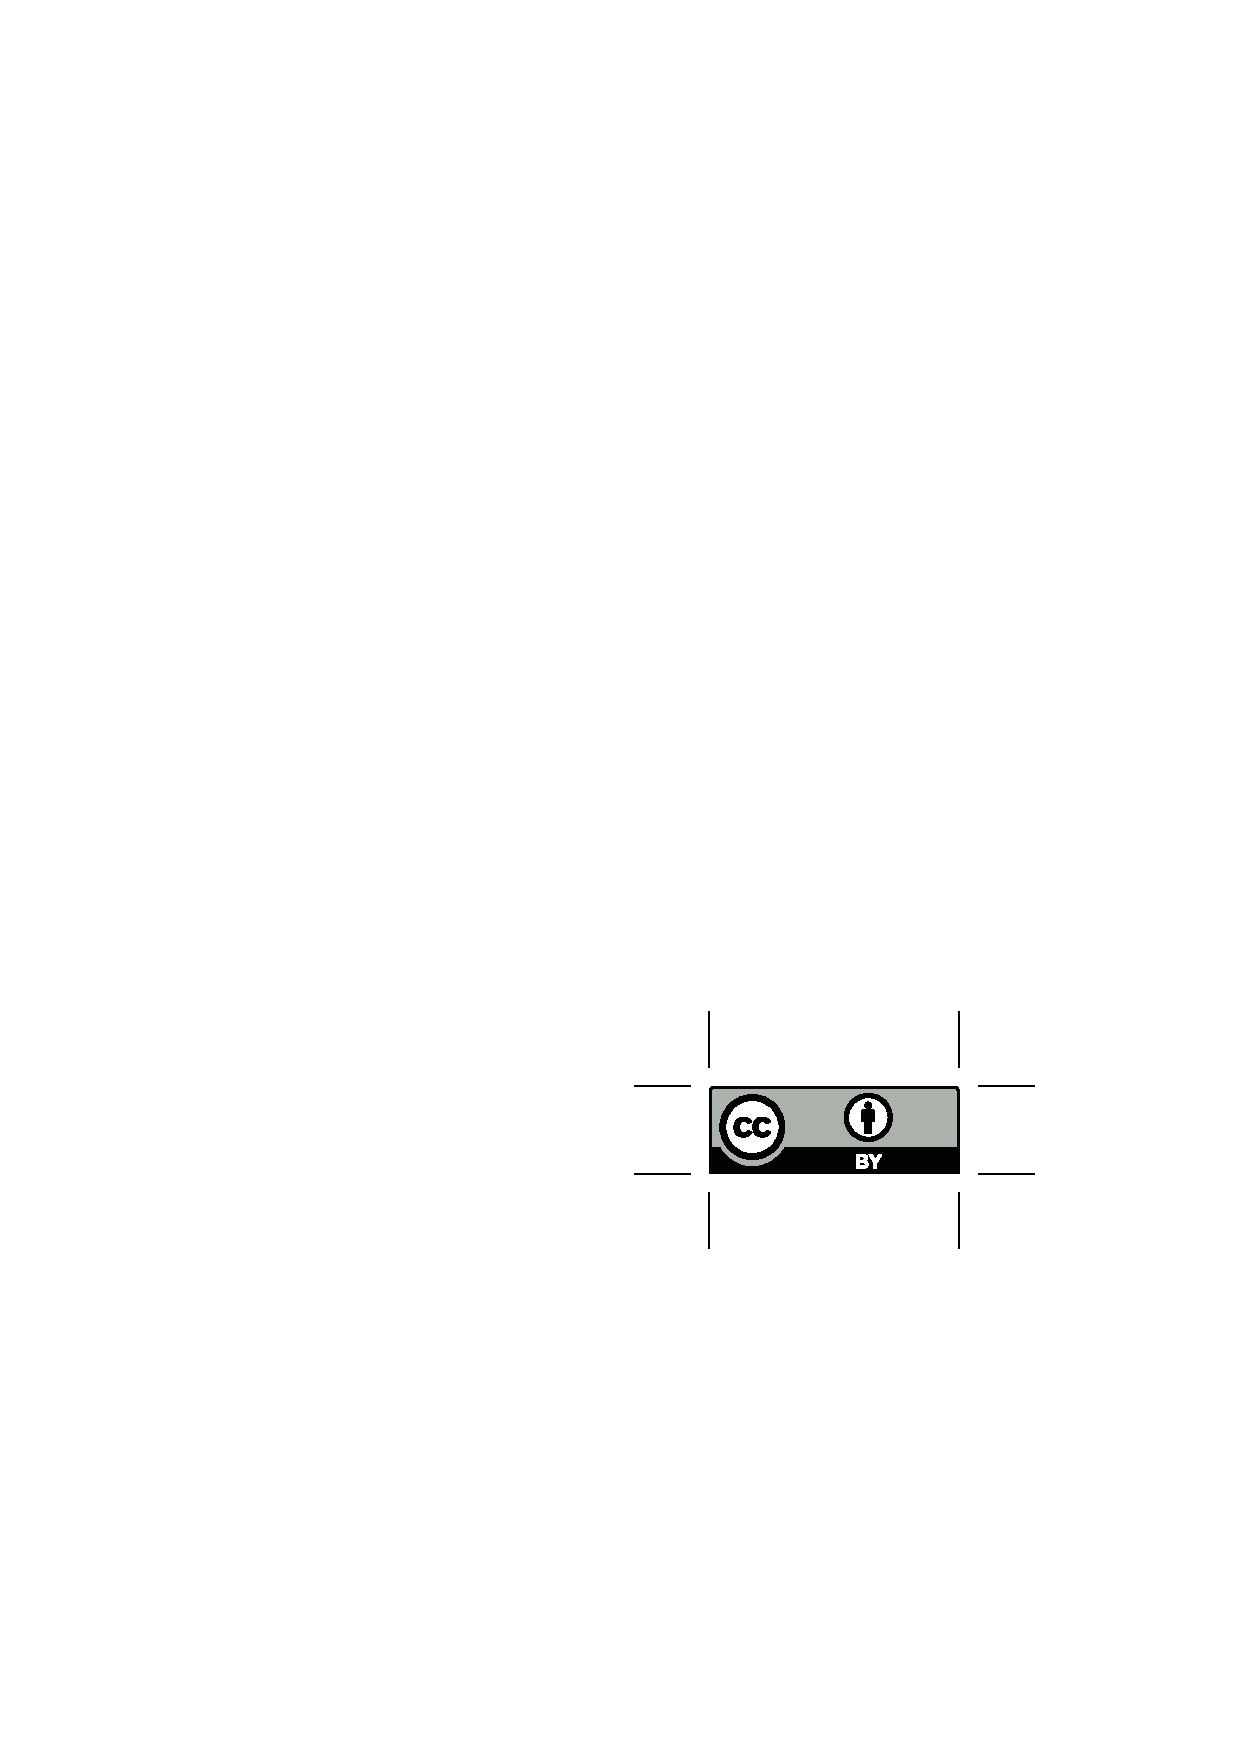
\includegraphics[height=14pt]{by} \\

{\tiny
This work is licensed under a
\href{http://creativecommons.org/licenses/by/4.0/}{Creative Commons Attribution 4.0 International License}.
}}

\begin{document}

\begin{frame}
  \titlepage
\end{frame}

\begin{frame} \frametitle{Big Idea: Algorithm Frameworks}
  \textbf{Algorithm framework:} an algorithm with modular parts that can be
    swapped in for different performance properties; or to solve different but
    related problems \stanza

  Example: hash tables are a framework, can swap in
  \begin{itemize}
    \item different collision resolution strategy (chaining, probing)
    \item different hash function (universal hash, linear congruential hash, etc.)
  \end{itemize}

  A framework generalizes several algorithm ideas into one pattern; ``chunking''
\end{frame}

\begin{frame} \frametitle{Big Idea: Iterative Pattern}
\begin{columns}
\begin{column}{0.5\textwidth}
Recall greedy pattern:
\begin{enumerate}
  \item initialize base-case result
  \item for each piece of input, update result
\end{enumerate}
\end{column}
\begin{column}{0.5\textwidth}
\textbf{Iterative pattern} (a.k.a. \emph{fixed-point algorithm}):
\begin{enumerate}
  \item initialize base-case result
  \item while result is not optimal:
  \begin{enumerate}
    \item improve result one step
  \end{enumerate}
\end{enumerate}
\end{column}
\end{columns}
\vspace{.5cm}
The \emph{fixed point} is the moment when the result becomes optimal. \stanza

Both use a \emph{greedy heuristic}; iterative pattern makes a problem-wide decision.
\end{frame}

\begin{frame} \frametitle{Big Idea: Problem Reduction}
\emph{problem $A$ reduces to problem $B$} $=$ can use an algorithm for $B$ to do all the hard
work of solving problem $A$ \\
$= A$ is easier than $B$ (or tied) \stanza

Sometimes $A, B$ are closely related \\
e.g. $A = $ sorting bounded integers, $B = $ general sorting \stanza

More interesting: problems seem completely unrelated (e.g. SAT, CLIQUE;
max-flow, bipartite matching)
\end{frame}

\begin{frame} \frametitle{Big Idea: Problem Duality}
\textbf{problem duality:} when the input/output mathematical definition of a
problem can be interpreted by humans in two (or more) very different ways
\begin{itemize}
  \item one algorithm can solve multiple problems with different ``stories''
  \item algorithms, computers, don't actually care what data values mean
  \item turns out max-flow and min-cut are two different stories for the same problem
  \item max-flow and min-cut are the \emph{dual of each other}
\end{itemize}
\end{frame}

\begin{frame} \frametitle{Duality Example}
\textbf{maximum $y$ coordinate} \\
\emph{input: } a set of $(x, y)$ points $S=\{(x, y) \, | \, x, y \in \mathbb{R} \}$ \\
\emph{output: } the greatext $y$-coordinate in $S$ \stanza

\textbf{highest $y$-intercept point problem} \\
\emph{input: } a set of $y=mx+b$ lines $L=\{(m, b) \, | \, m, b \in \mathbb{R} \}$ \\
\emph{output: } the greatext $y$-intercept $b$ in $L$ \stanza
\end{frame}

\begin{frame} \frametitle{Geometry Sketch}
\begin{center}
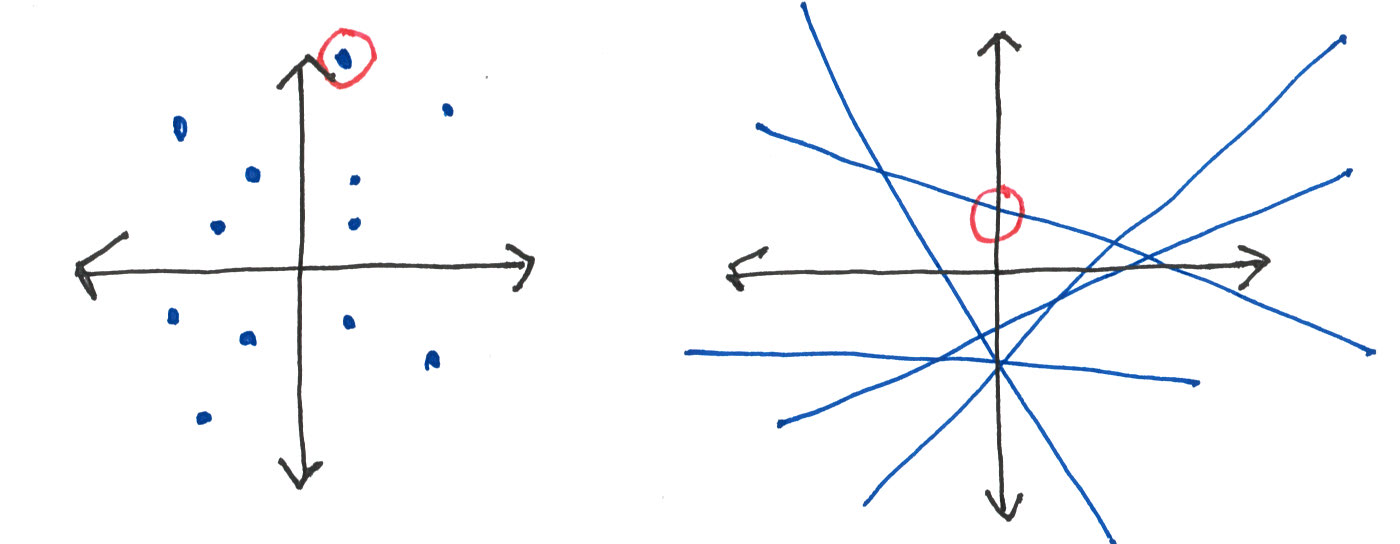
\includegraphics{lines.png}
\end{center}
\end{frame}

\begin{frame} \frametitle{}
C++ functions for these would be declared like:
\lstinline!double maximum_y_coord(vector<pair<double, double>>& points);!
\lstinline!double highest_y_intercept(vector<pair<double, double>>& lines);! \stanza

As far as the computer is concerned, these are interchangeable! \stanza

Only the human story differs.
The
\textbf{maximum $y$ coordinate}
and
\textbf{highest $y$-intercept point problem}
problems are the dual of each other.
\end{frame}

\begin{frame} \frametitle{Defining Maximum Flow 1/2: Flow Networks}
\emph{flow network:} graph representing resource flows
\begin{itemize}
  \item directed graph $G=(V, E)$
  \item designated \emph{source vertex} $s \in V$ and \emph{sink vertex} $t \in V$
  \item \textbf{no self-loop}: $\forall v \in V$, $(v, v) \notin E$
  \item \textbf{no antiparallel edges}: for any $\forall (u, v) \in E, (v, u) \notin E$
  \item flow is possible through every vertex: $\forall v \in V,$ there exists
    some path $s \leadsto v \leadsto t$
  \item \emph{capacity:} $\forall (u, v) \in E,$ there is a defined,
    non-negative real capacity $c(u, v)$
  \item implies: $G$ is connected and $|E| \geq |V|-1$
\end{itemize}
\end{frame}

\begin{frame} \frametitle{Flow Network Sketches}
\begin{center}
  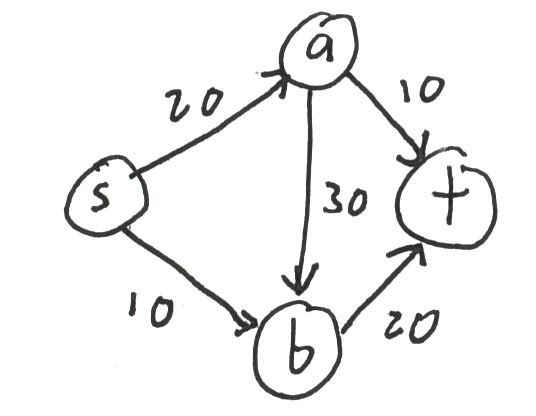
\includegraphics[height=1.5in]{flownetwork-1.png} 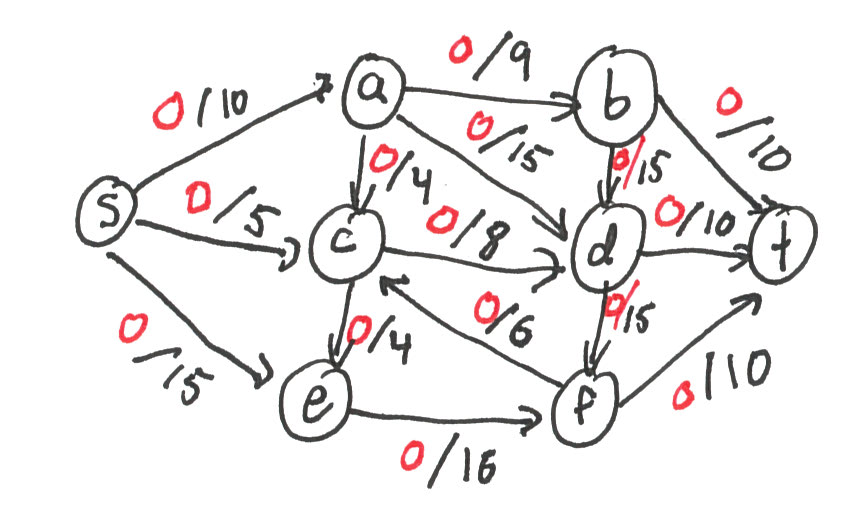
\includegraphics[height=1.5in]{flownetwork-2.png}
\end{center}
\end{frame}

\begin{frame} \frametitle{Defining Maximum Flow 2/2: Flows}
\emph{flow:} settings for how much capacity to use on each edge
\begin{itemize}
  \item candidate for maximum flow: follows the ``rules,'' but not necessarily
    optimal
  \item modeled as function $f(u, v)$ over vertices $u, v$
  \item \textbf{nonexistent edges}: if $(u, v) \notin E$ then $f(u, v) = 0$
  \item \textbf{capacity constraint}: $0 \leq f(u, v) \leq c(u, v)$
  \item \textbf{flow conservation}: (flow-in) $=$ (flow-out), except for source and
    sink; formally, $\forall u \in V - \{s, t\},$
    \[ \sum_{v \in V} f(v, u) = \sum_{v \in V} f(u, v) \]
  \item \emph{value} $|f|$ = net flow into sink
    \[ |f| = \sum_{v \in V} f(s, v) - \sum_{v \in V} f(v, s) \]
\end{itemize}
\end{frame}

\begin{frame} \frametitle{Flow Sketch}
\begin{center}
  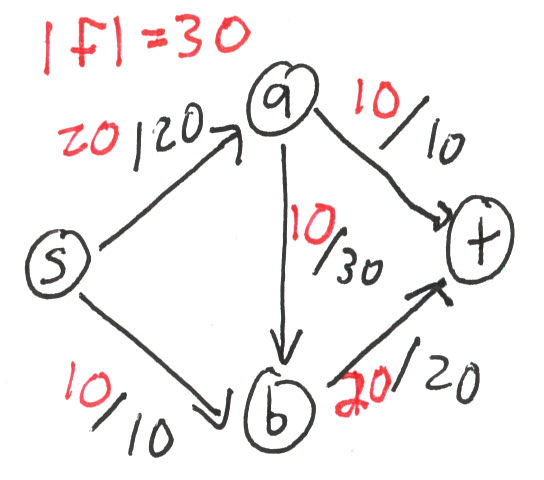
\includegraphics{flow-example.png}
\end{center}
\end{frame}

\begin{frame} \frametitle{Maximum Flow Problem Definition}
\textbf{maximum flow problem} \\
\emph{input:} a flow network $G$ \\
\emph{output:} a flow $f$ of maximum value $|f|$ \stanza
\end{frame}

\begin{frame} \frametitle{Ford-Fulkerson Method}
``method'' because this is a pattern for specific max-flow algorithms
\begin{itemize}
  \item not a complete, clear alg. yet
  \item based on iterative improvement pattern \stanza
\end{itemize}

{\footnotesize
\begin{algorithmic}[1]
  \Function{ITERATIVE-IMPROVEMENT}{input}
  \State result = base-case result
  \While { result is not optimal }
    \State improve result
  \EndWhile
  \State \Return { result }
  \EndFunction
\end{algorithmic}
}

\end{frame}

\begin{frame} \frametitle{Ford-Fulkerson Method}
{\footnotesize
\begin{algorithmic}[1]
  \Function{FORD-FULKERSON-METHOD}{$G, s, t$}
  \State $f$ = flow with every edge set to zero
  \State initialize residual network $G_f$
  \While { there exists an augmenting path $p$ in $G_f$ }
    \State augment flow $f$ along path $p$
  \EndWhile
  \State \Return { $f$ }
  \EndFunction
\end{algorithmic}
}
\vspace{.5cm}

Need to explain
\begin{itemize}
  \item \emph{residual network}
  \item \emph{augmenting path}
  \item why this terminates and is correct
\end{itemize}
\end{frame}

\begin{frame} \frametitle{Residual Networks}
\begin{itemize}
  \item residual network $G_f$ has same vertices as flow network $G=(V,E)$
  \item edges reflect how much capacity is still available
  \item $G_f$ only contains edges with positive available capacity
  \item also add ``backwards'' edges to allow us to take-back some positive flow
  \item define \emph{residual capacity} between vertices $v, w \in V$ as
\end{itemize}

  \[
      c_f(u, v) =
      \begin{cases}
        c(u, v) - f(u, v) & \text{if } (u, v) \in E \\
        f(v, u) & \text{if } (v, u) \in E \\
        0 & \text{otherwise}
      \end{cases}
  \]

\begin{itemize}
  \item (recall that in a flow network either $(u, v) \in E$ or $(v, u) \in E$
    but not both)
\end{itemize}
\end{frame}

\begin{frame} \frametitle{Residual Network Example}
  \begin{center}
    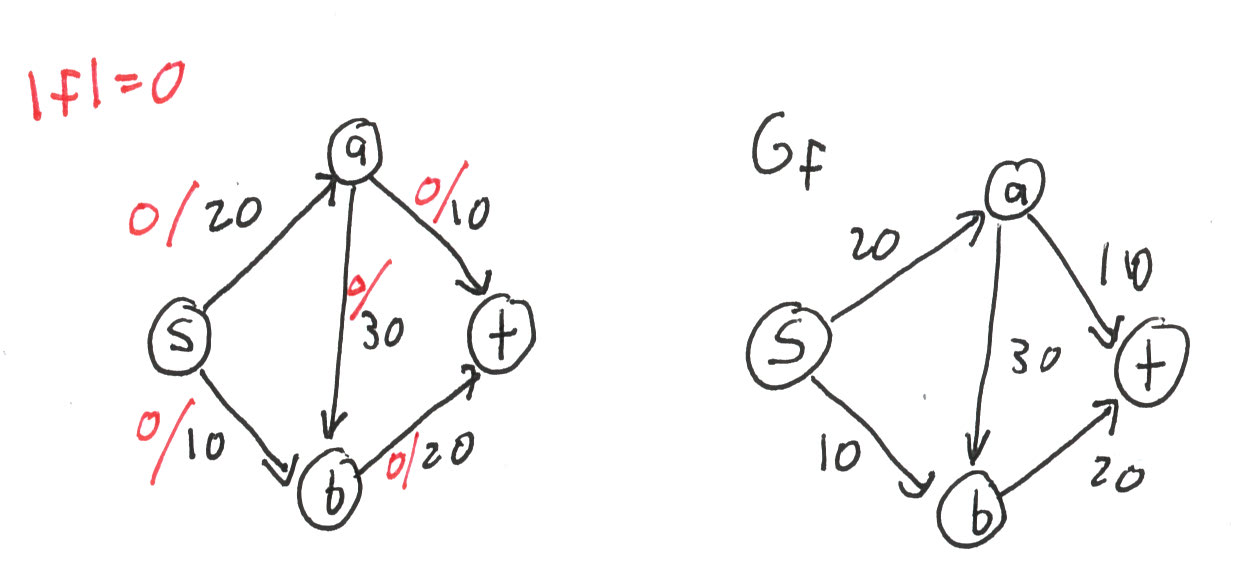
\includegraphics[scale=.6]{residual-1.png} \\

    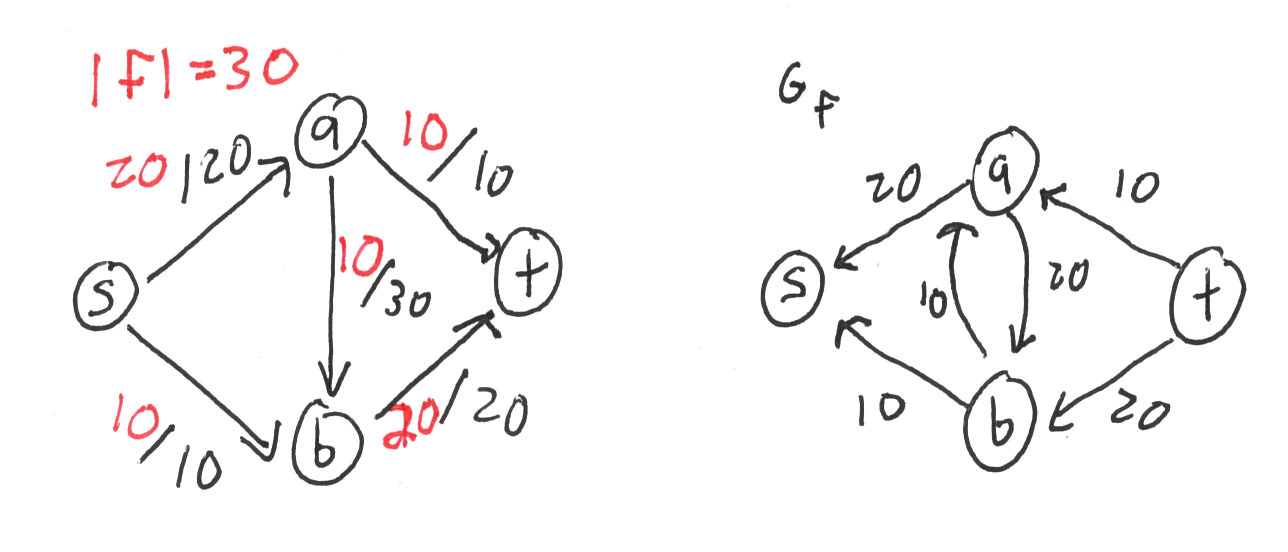
\includegraphics[scale=.6]{residual-2.png}
  \end{center}
\end{frame}

\begin{frame} \frametitle{Augmenting Paths}
\begin{itemize}
  \item \emph{augmenting path:} simple path from source $s$ to sink $t$ in residual
    network $c_f$
    (\emph{simple} $\equiv$ no repeated vertices)
  \item recall: residual network $G_f$ only contains edges with leftover capacity
  \item $\implies$ if path $p$ exists in $G_f,$ then every edge along $p$
    has positive weight in $G_f$
  \item $\implies$ we can legally increase net $s \leadsto t$ flow by increasing
    weights in $G_f$
  \item i.e. increasing flow across the forwards edges in $G_f,$ sometimes
    decreasing flow acress the backwards edges
  \item $c_f(p) = $\emph{residual capacity} of $p$ = minimum weight
    $c_f(u,v)$ of an edge $(u, v)$ in $p$
\end{itemize}
\end{frame}

\begin{frame} \frametitle{Ford-Fulkerson Method Recap}
Recall the Ford-Fulkerson method/pattern:
{\footnotesize
\begin{algorithmic}[1]
  \Function{FORD-FULKERSON-METHOD}{$G, s, t$}
  \State $f$ = flow with every edge set to zero
  \State initialize residual network $G_f$
  \While { there exists an augmenting path $p$ in $G_f$ }
    \State augment flow $f$ along path $p$
  \EndWhile
  \State \Return { $f$ }
  \EndFunction
\end{algorithmic}
}
\vspace{.5cm}
still need to
\begin{itemize}
  \item clarify how to pick $p$: modular choice leading to specific algorithms
  \item prove correctness and termination: \emph{max-flow min-cut theorem}
\end{itemize}
\end{frame}

\begin{frame} \frametitle{Max-Flow Min-Cut Theorem}
Lemma: Augmenting a flow $f$ with path $p$ increases $s \leadsto t$ flow by $c_f(p).$
\stanza

\textbf{Max-Flow Min-Cut Theorem:} flow $f$ is maximum iff $G_f$ contains no augmenting path.
\stanza

If true, any Ford-Fulkerson algorithm computes a correct maximum flow.

But,
\begin{itemize}
  \item does not imply that the algorithm terminates
  \item does not imply that the \# loop iterations is small
  \item need to decide how to pick paths carefully
  \item we'll come back to this later
\end{itemize}
\end{frame}

\begin{frame} \frametitle{Cuts}
\begin{itemize}
  \item \emph{cut:} partition $V=S \cap T,$ where $s \in S$ and $t \ in T$
  \item \emph{net flow} across $f$ is
    \[ f(S, T) = (\text{total flow from } S \text{ to } T) -
                  (\text{flow from } T \text{ to } S) \]
  \item \emph{minimum cut} = a cut whose net flow is minimum
\end{itemize}
\vspace{.5cm}

Lemma: for any cut $(S, T)$, net flow $f(S,T) = |f|.$ \\
Proof sketch: since $s \in S$ and $t \in T,$ total flow $|f|$ must cross the
$S$--$T$ boundary.
\end{frame}

\begin{frame} \frametitle{Max-Flow Min-Cut Proof Sketch}
Show all these are equivalent conditions:
\begin{enumerate}
  \item $f$ is a maximum flow
  \item $G_f$ contains no augmenting path
  \item $|f| = c(S, T)$ for some cut $(S, T)$
\end{enumerate}

$(1) \implies (2):$ by definitions of residual network and augmenting path,
a maximum flow has no capacity leftover so no paths in $G_f$ \stanza

$(2) \implies (3):$ consider a cut where all vertices reachable from $s$ in $G_f$
are in $S$ and the unreachables are in $T$; since there is no $s \leadsto t$
path in $G_f,$ all edges across the $S$--$T$ boundary must already be at full capacity
\stanza

$(3) \implies (1)$: trivially $|f| \leq c(S, T)$, and if $|f|=c(S, T)$ then this
$(S, T)$ is maximum
\end{frame}

\begin{frame} \frametitle{Ford-Fulkerson Detailed Pseudocode}
{\footnotesize
\begin{algorithmic}[1]
  \Function{FORD-FULKERSON-METHOD}{$G=(V, E), s, t$}
  \For { each edge $(u, v)$ in $E$ }
    \State $(u, v).f = 0$
  \EndFor
  \While { there exists an augmenting path $p$ in $G_f$ }
    \State $c_f(p) = \min\{c_f(u, v) : (u, v) \in p\}$
    \For { each edge $(u, v) \in p$ }
      \If { $(u, v) \in E$ }
        \State $(u, v).f = (u, v).f + c_f(p)$
      \Else
        \State $(u, v).f = (v, u).f + c_f(p)$
      \EndIf
    \EndFor
  \EndWhile
  \State \Return { flow on $.f$ fields }
  \EndFunction
\end{algorithmic}
}
Still abstract --- need to clarify how we choose path $p.$
\end{frame}

\begin{frame} \frametitle{Edmonds-Karp Algorithm}
Edmonds-Karp Algorithm is
\begin{itemize}
  \item Ford-Fulkerson method from previous page, and...
  \item use breadth-first search (BFS) to find the shortest augmenting path
  \item (shortest $\equiv$ fewest vertices, irrespective of weights)
  \item now a concrete, runnable, implementable algorithm
  \item performs $O(|V| \cdot |E|)$ augmentations
  \item takes $O(|V| \cdot |E|^2)$ time
  \item for $n=|V|$, this is $O(n^3)$ in a sparse graph and $O(n^5)$ in a dense graph
  \item more complicated \textbf{relabel-to-front} algorithm takes $O(|V|^3)=O(n^3)$
    time
\end{itemize}
\end{frame}

\begin{frame} \frametitle{Edmonds-Karp Pseudocode for Worked Examples}
  {\footnotesize
  \begin{algorithmic}[1]
    \Function{EDMONDS-KARP}{$G=(V, E), s, t$}
    \State initialize each edge's capacity to 0
    \Repeat
      \For{ $k = 2, 3, \ldots, |V|$ }
        \If { $\exists \text{ augmenting path } p \text { of length k }$ }
          \State $c_f(p)$ = minimum excess capacity of any edge in $p$
          \For { edge $e$ in $p$ }
            \If { $p$ follows $e$ forwards }
              \State increase $e$'s flow by $c_f(p)$
            \Else
              \State decrease $e$'s flow by $c_f(p)$
            \EndIf
          \EndFor
          \State break loop
        \EndIf
      \EndFor
    \Until { no path can be found }
    \State \Return { flow based on current capacities }
    \EndFunction
  \end{algorithmic}
  }
\end{frame}

\begin{frame} \frametitle{Identifying Edge Capacity in $G$}
When running this algorithm by hand,
\begin{itemize}
  \item you \emph{could} sketch the residual network each time, but this is tedious
  \item instead, when looking at edge $e$ with flow $x/c$
  \item if $x<c,$ you \emph{may} follow $e$ forwards and add up to $(c-x)$ flow
  \item if $x>0,$ you \emph{may} follow $e$ backwards and subtract up to $x$ flow
\end{itemize}
\end{frame}

\begin{frame} \frametitle{Edmonds-Carp Example 1/2}
\begin{center}
  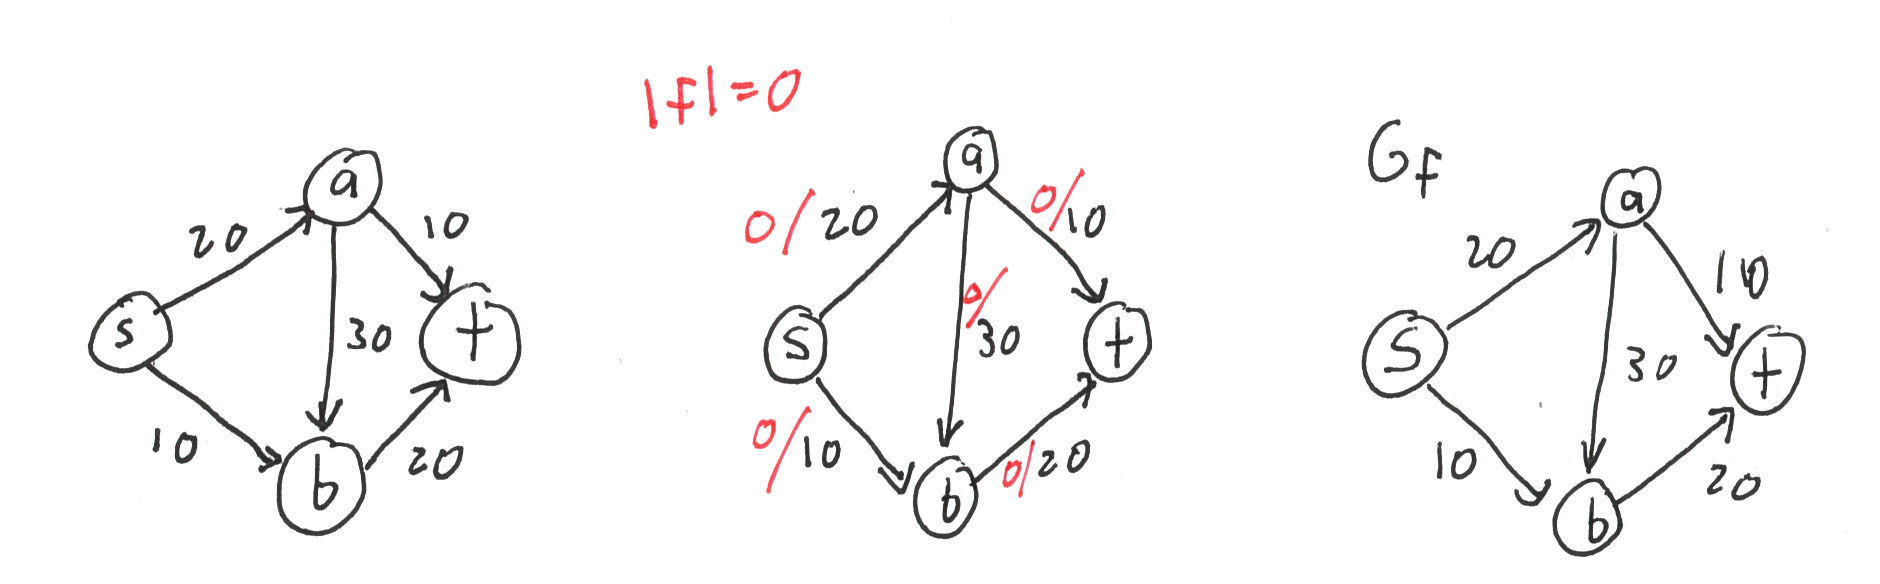
\includegraphics[scale=.6]{ek-1-1.png}
\end{center}
\end{frame}

\begin{frame} \frametitle{Edmonds-Carp Example 1/2}
\begin{center}
  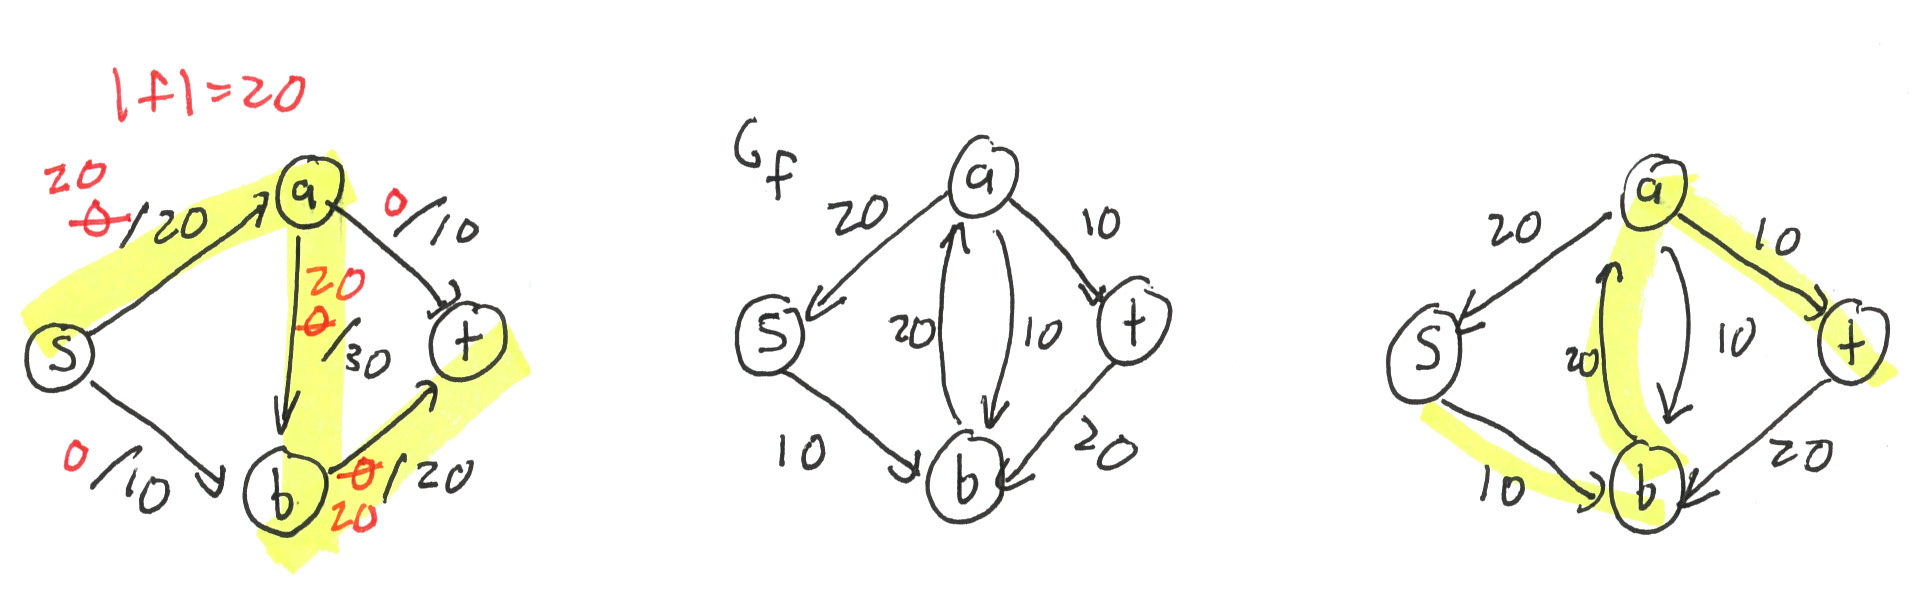
\includegraphics[scale=.6]{ek-1-2.png}
\end{center}
\end{frame}

\begin{frame} \frametitle{Edmonds-Carp Example 2/2}
\begin{center}
  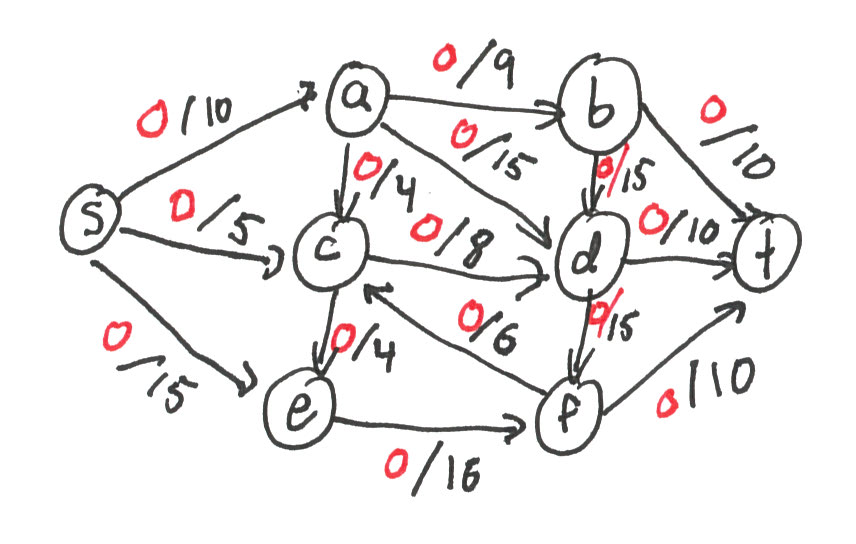
\includegraphics[scale=1]{ek-2-1.png}
\end{center}
\end{frame}

\begin{frame} \frametitle{Edmonds-Carp Example 2/2}
\begin{center}
  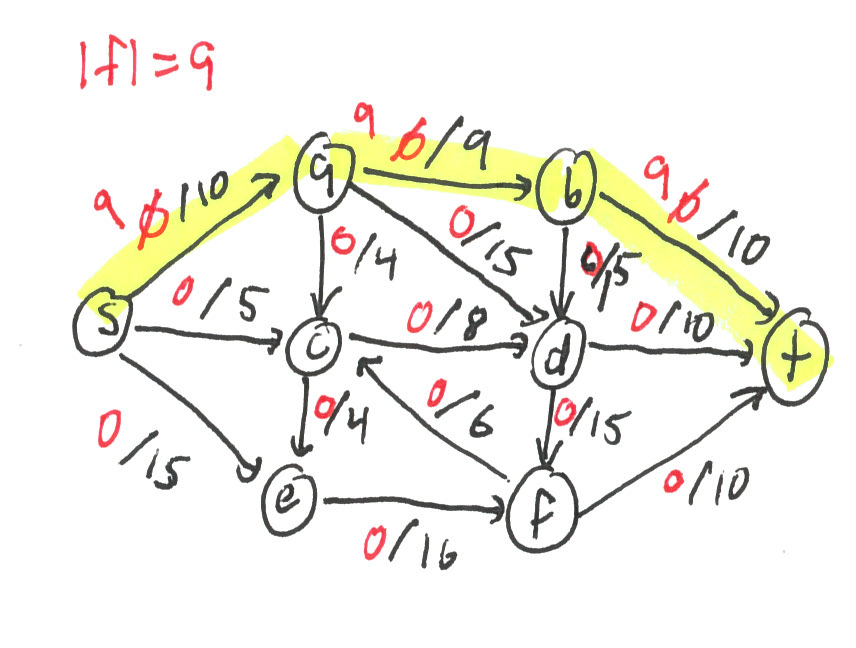
\includegraphics[scale=1]{ek-2-2.png}
\end{center}
\end{frame}

\begin{frame} \frametitle{Edmonds-Carp Example 2/2}
\begin{center}
  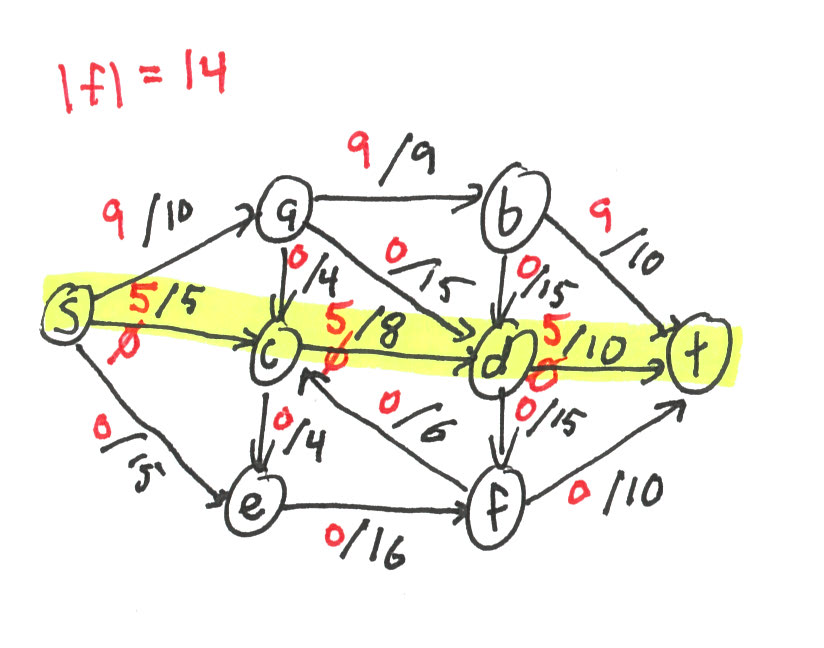
\includegraphics[scale=1]{ek-2-3.png}
\end{center}
\end{frame}

\begin{frame} \frametitle{Edmonds-Carp Example 2/2}
\begin{center}
  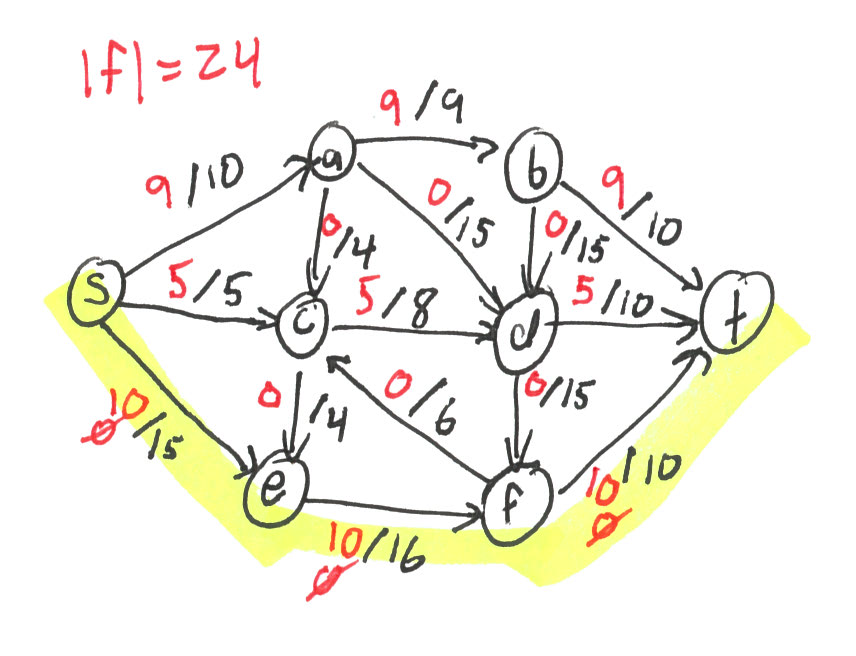
\includegraphics[scale=1]{ek-2-4.png}
\end{center}
\end{frame}

\begin{frame} \frametitle{Edmonds-Carp Example 2/2}
\begin{center}
  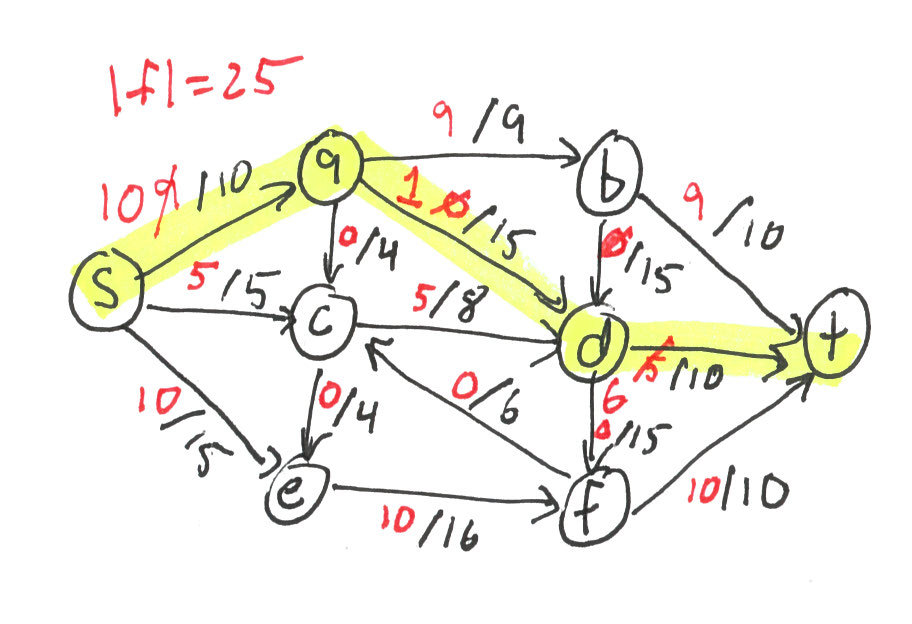
\includegraphics[scale=1]{ek-2-5.png}
\end{center}
\end{frame}

\begin{frame} \frametitle{Edmonds-Carp Example 2/2}
\begin{center}
  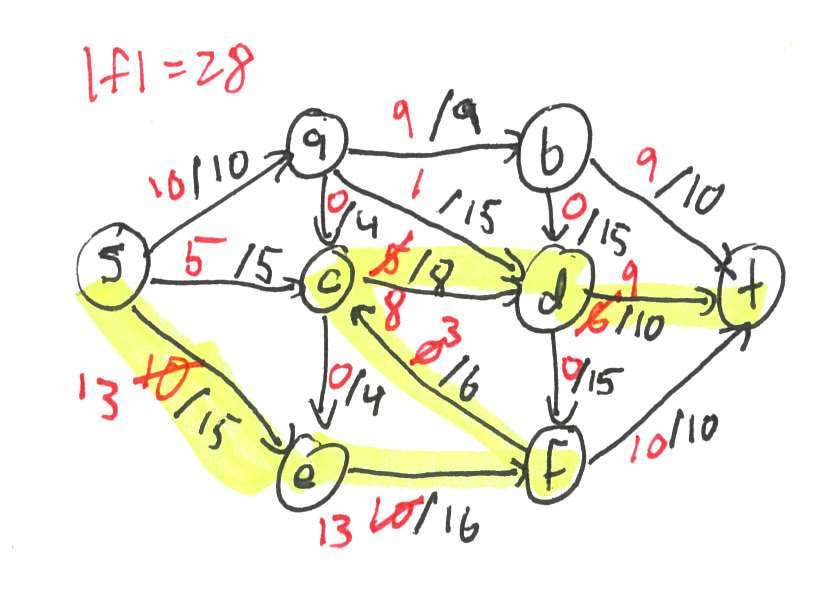
\includegraphics[scale=1]{ek-2-6.png}
\end{center}
\end{frame}

\begin{frame} \frametitle{Edmonds-Carp Example 2/2}
\begin{center}
  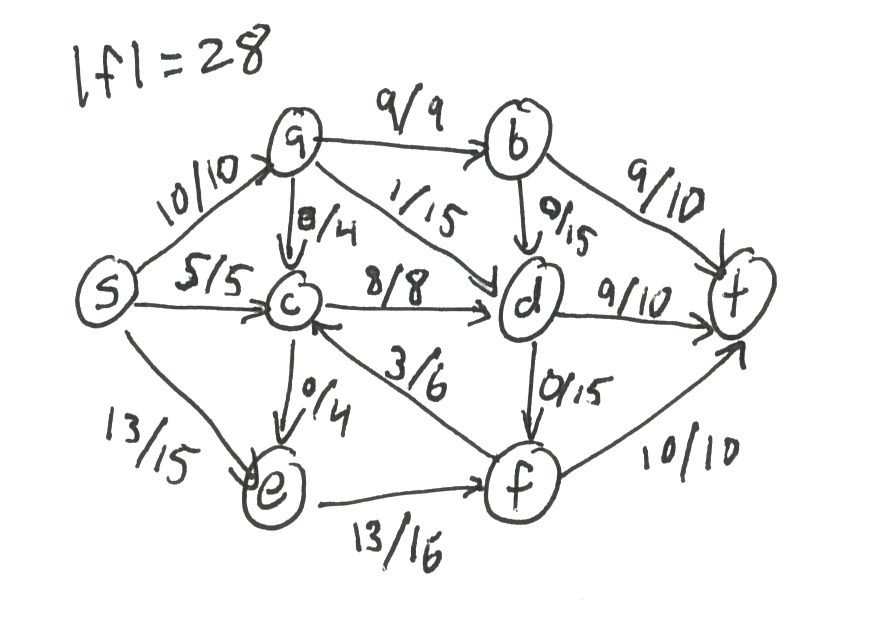
\includegraphics[scale=1]{ek-2-7.png}
\end{center}
\end{frame}


\end{document}
